
\section{Tafel ronde 2: Wie is het?}
Freddy heeft een paar mooie foto's gevonden van het home Astrid presidium. Kan jij raden wie het is?

Enkel voornaam, fonentisch geschreven
\begin{questions}
\question[1] {
\begin{center}
{
\includegraphics[scale=0.20]{robbe}}
\end{center}
\begin{flushleft}
\makebox[\textwidth]{naam:\enspace\hrulefill}
\end{flushleft} }
\question[1] {
\begin{center}
{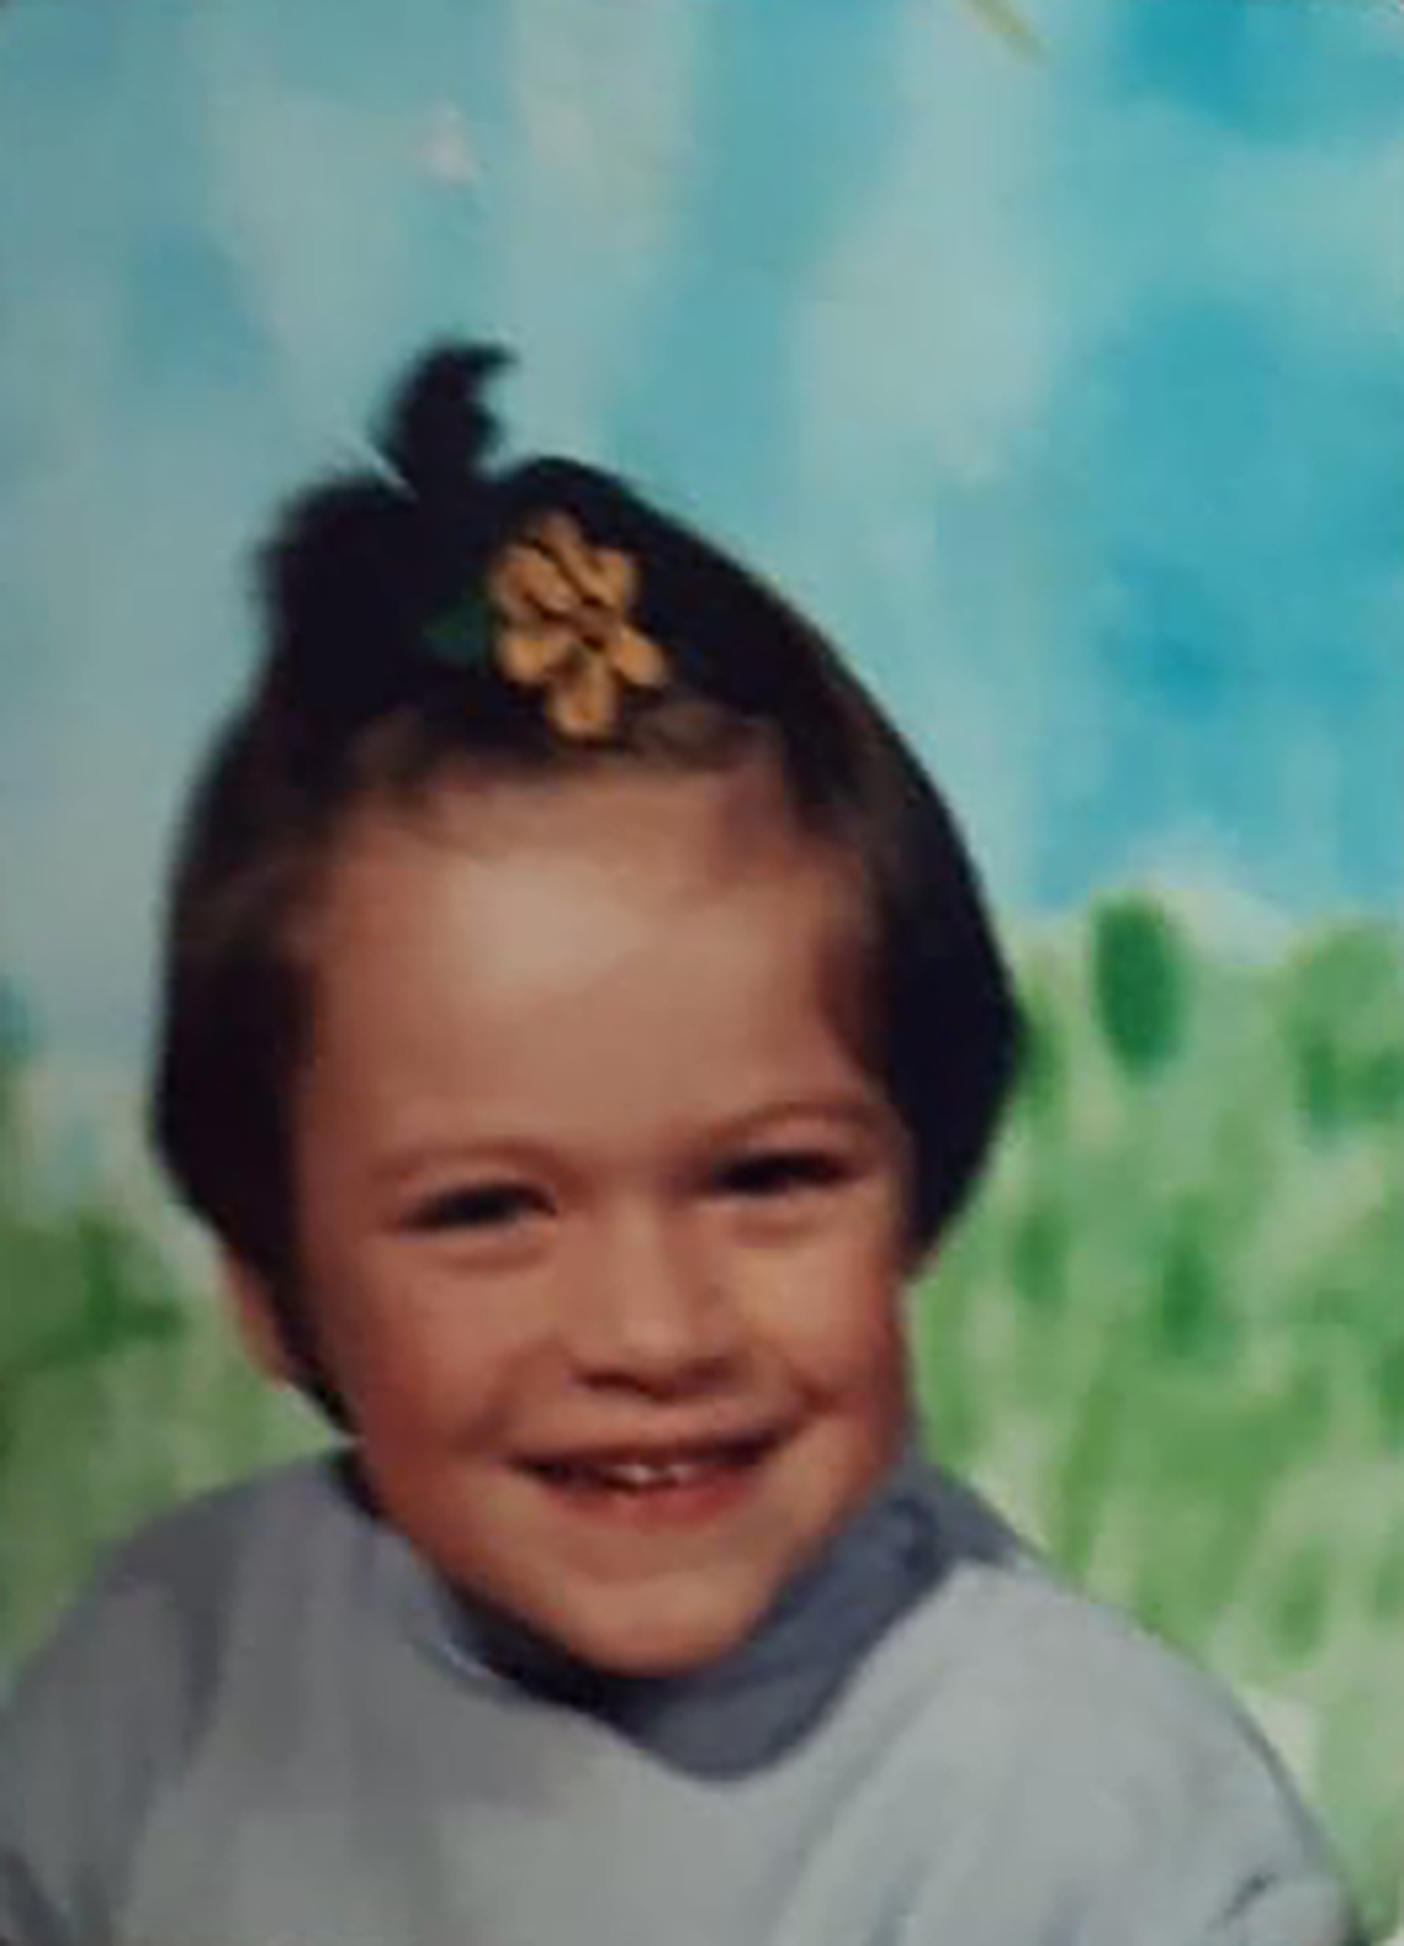
\includegraphics[scale=0.08]{lisa}}
\end{center}
\begin{flushleft}
\makebox[\textwidth]{naam:\enspace\hrulefill}
\end{flushleft} }
\question[1] {
\begin{center}
{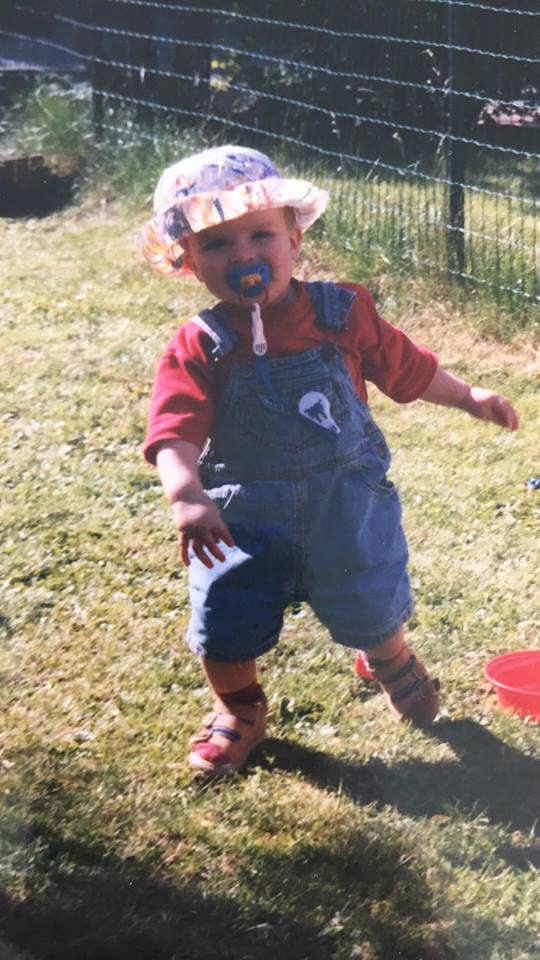
\includegraphics[scale=0.20]{arend}}
\end{center}
\begin{flushleft}
\makebox[\textwidth]{naam:\enspace\hrulefill}
\end{flushleft} }
\question[1] {
\begin{center}
{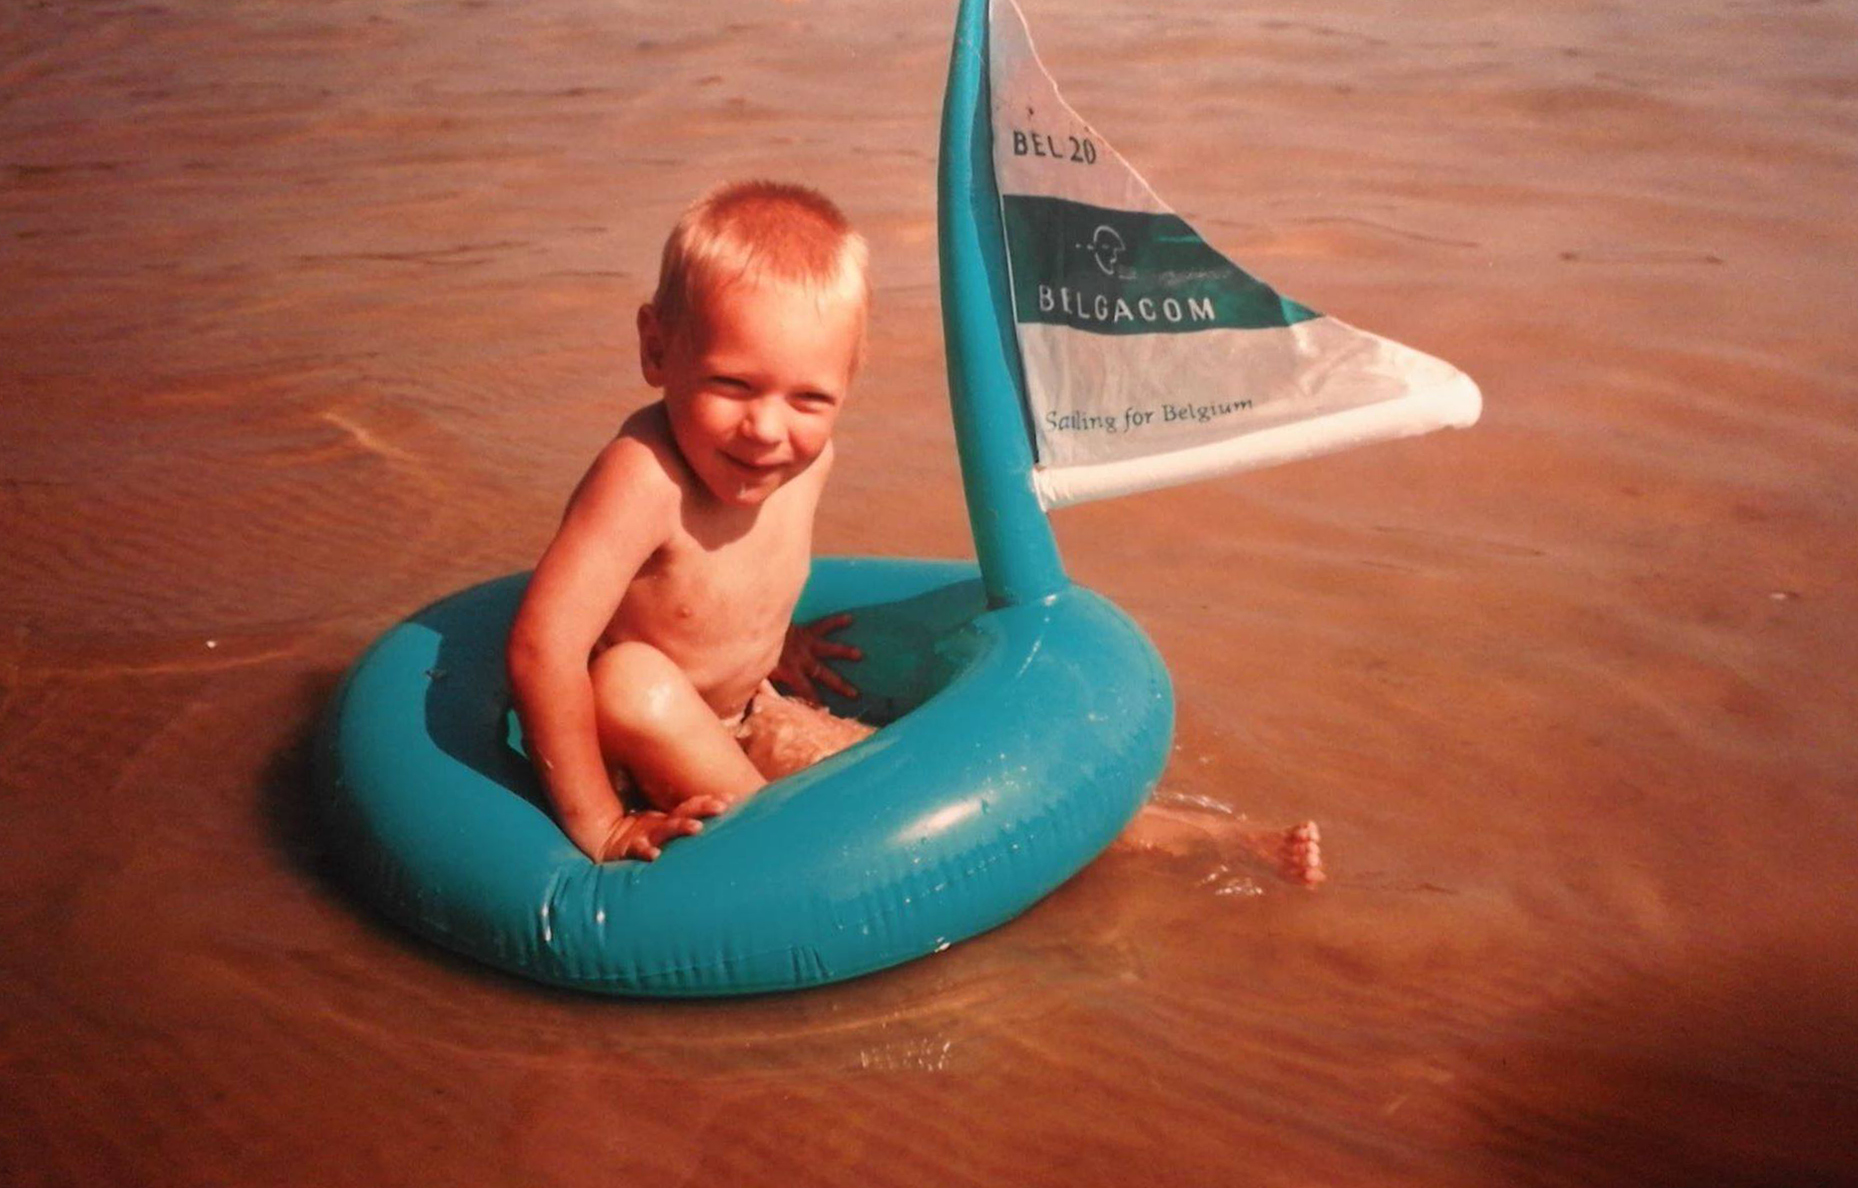
\includegraphics[scale=0.10]{bart}}
\end{center}
\begin{flushleft}
\makebox[\textwidth]{naam:\enspace\hrulefill}
\end{flushleft} }
\question[1] {
\begin{center}
{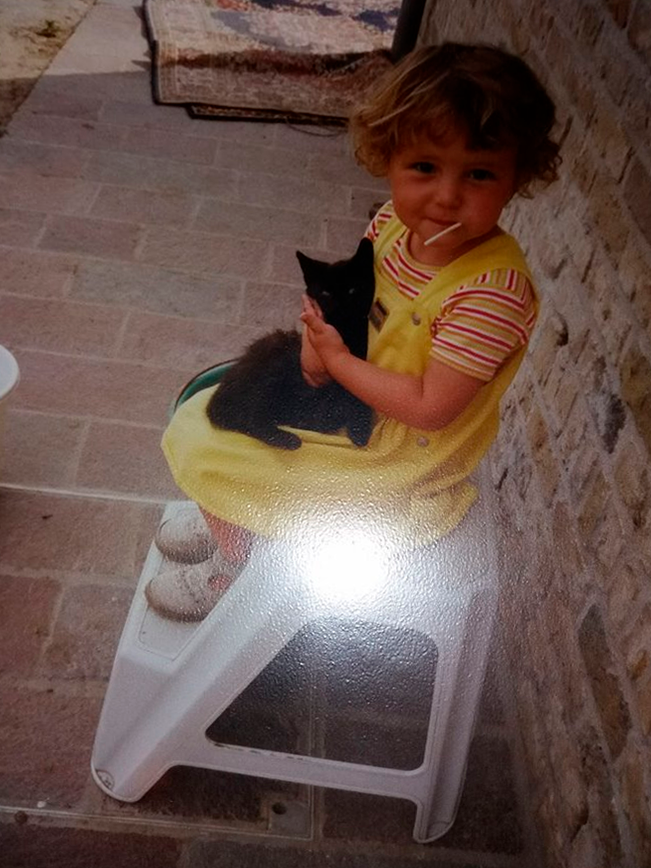
\includegraphics[scale=0.20]{michelle}}
\end{center}
\begin{flushleft}
\makebox[\textwidth]{naam:\enspace\hrulefill}
\end{flushleft} }
\question[1] {
\begin{center}
{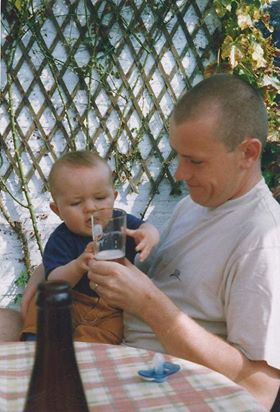
\includegraphics[scale=0.40]{lemmy}}
\end{center}
\begin{flushleft}
\makebox[\textwidth]{naam:\enspace\hrulefill}
\end{flushleft} }
\question[1] {
\begin{center}
{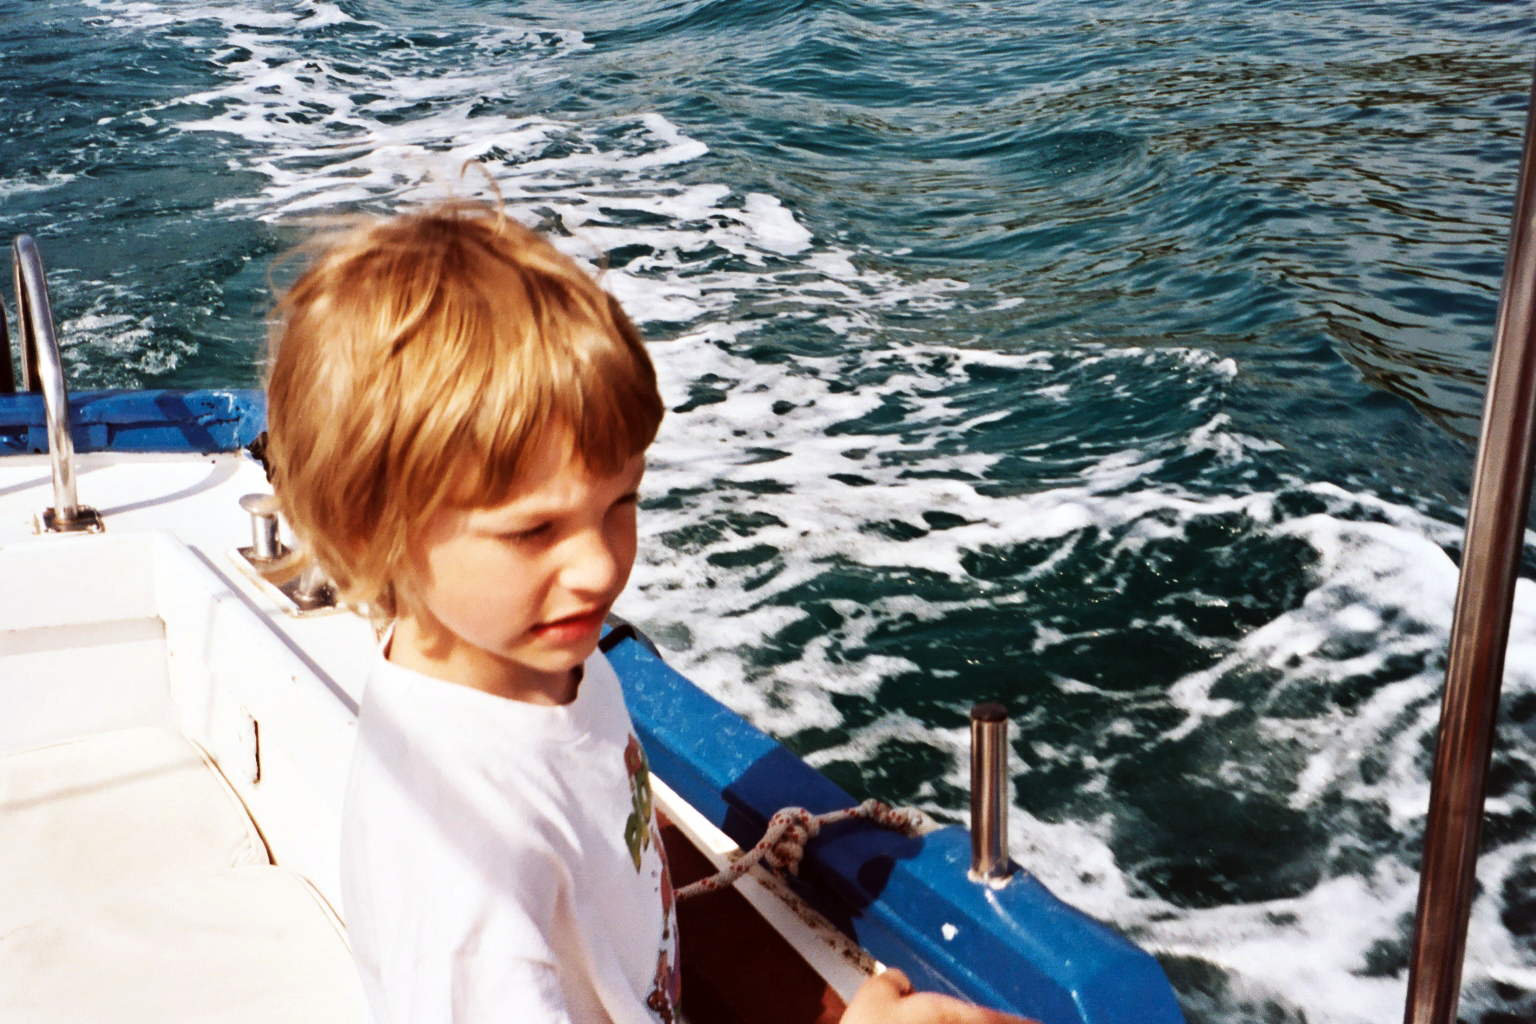
\includegraphics[scale=0.40]{tibo}}
\end{center}
\begin{flushleft}
\makebox[\textwidth]{naam:\enspace\hrulefill}
\end{flushleft} }
\question[1] {
\begin{center}
{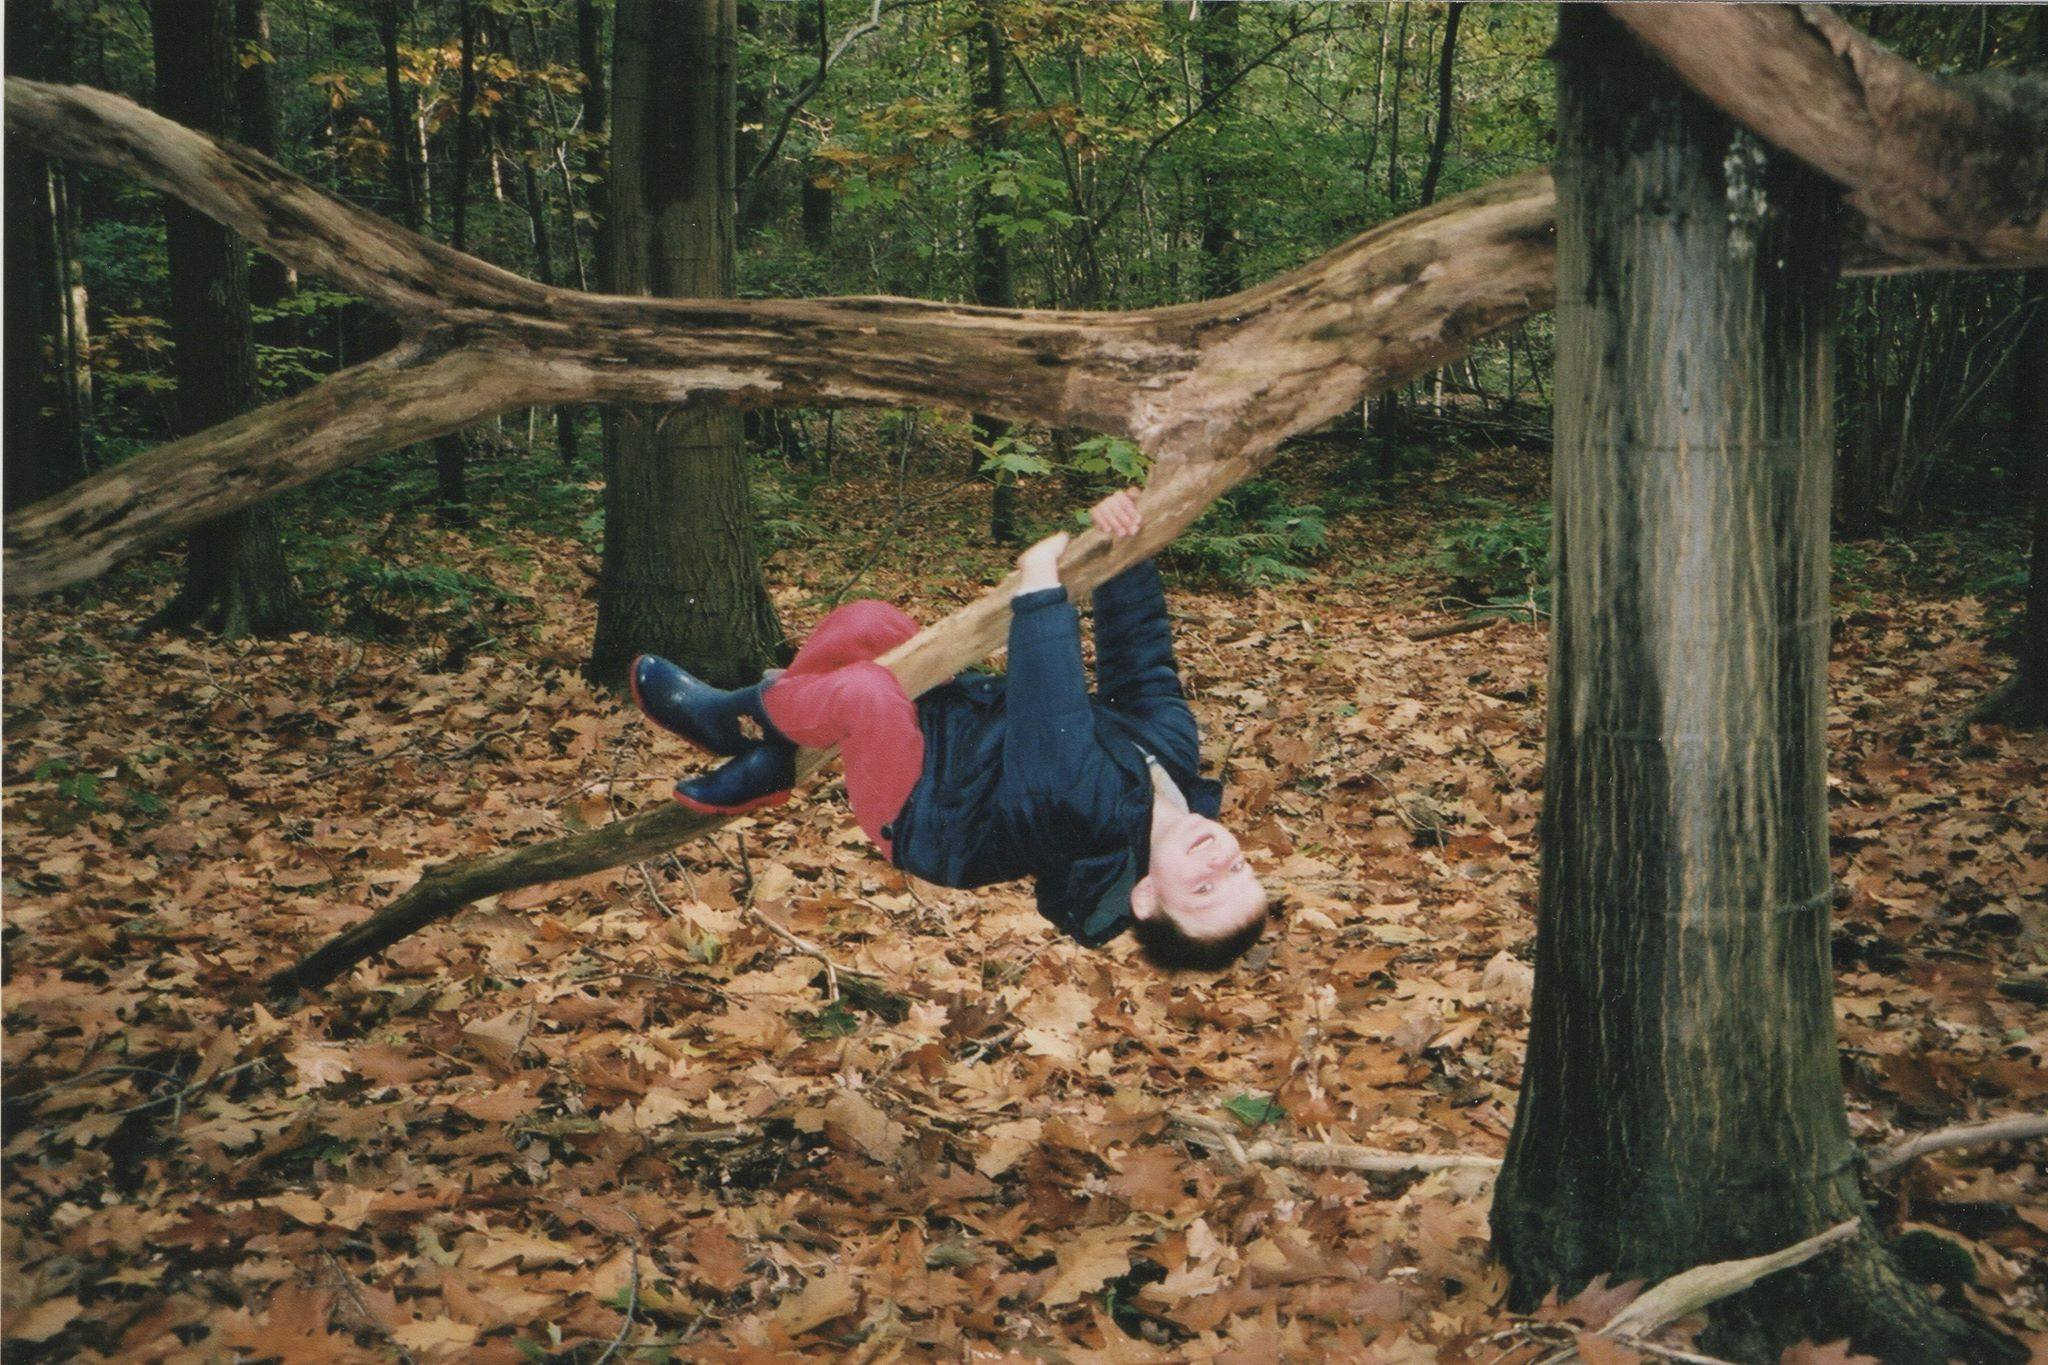
\includegraphics[scale=0.10]{wouter}}
\end{center}
\begin{flushleft}
\makebox[\textwidth]{naam:\enspace\hrulefill}
\end{flushleft} }
\question[1] {
\begin{center}
{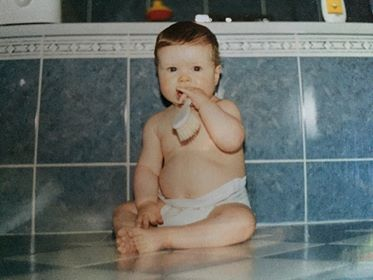
\includegraphics[scale=0.40]{elien}}
\end{center}
\begin{flushleft}
\makebox[\textwidth]{naam:\enspace\hrulefill}
\end{flushleft} }
\question[1] {
\begin{center}
{
\includegraphics[scale=0.10]{sander}}
\end{center}
\begin{flushleft}
\makebox[\textwidth]{naam:\enspace\hrulefill}
\end{flushleft} }

\end{questions}

\begin{table}[!b]
\centering
\begin{tabular}{|l|l|l|l|l|l|l|l|l|l|l|l}
\hline
Vraag       & 1 & 2 & 3 & 4 & 5 & 6 & 7 & 8 & 9 & 10 \\ \hline
max. punten & 1 & 1 & 1 & 1 & 1 & 1 & 1 & 1 & 1 & 1 \\ \hline
score       &   &   &   &   &   &   &   &   &   &   \\ \hline
\end{tabular}
\end{table}
\newpage